\documentclass[11pt,a4paper]{article}

% ---------------------------------------------------------------- packages
\usepackage[margin=0.75in]{geometry}
\usepackage{newtxtext,newtxmath}
\usepackage[T1]{fontenc}
\usepackage{graphicx}
\usepackage{booktabs}
\usepackage{tabularx}
\usepackage{array}
\usepackage{multirow}
\usepackage{float}
\usepackage{caption}
\usepackage{subcaption}
\usepackage{enumitem}
\usepackage{xcolor}
\usepackage{listings}
\usepackage{titlesec}
\usepackage{tikz}
\usetikzlibrary{positioning,arrows.meta}
\usepackage[hidelinks]{hyperref}

\captionsetup{font=small,labelfont=bf}
\setlist{itemsep=2pt,topsep=4pt}
\setlength{\parskip}{4pt}
\setlength{\parindent}{0pt}
\renewcommand{\arraystretch}{1.15}

% Headings in the style of the department's lab reports: bold serif,
% main headings centred.
\titleformat{\section}{\centering\large\bfseries\MakeUppercase}{\thesection.}{0.5em}{}
\titleformat{\subsection}{\normalsize\bfseries}{\thesubsection}{0.6em}{}
\titleformat{\subsubsection}{\normalsize\bfseries\itshape}{\thesubsubsection}{0.6em}{}
\titlespacing*{\section}{0pt}{14pt}{8pt}
\titlespacing*{\subsection}{0pt}{10pt}{4pt}

\lstset{basicstyle=\ttfamily\small,frame=single,framerule=0.4pt,
        rulecolor=\color{black!40},columns=fullflexible,breaklines=true,
        xleftmargin=4pt,xrightmargin=4pt,aboveskip=6pt,belowskip=6pt}

\newcolumntype{Y}{>{\centering\arraybackslash}X}

\begin{document}

% ================================================================ cover
\pagenumbering{gobble}
\begin{titlepage}
\centering
\vspace*{0.4cm}
{\LARGE\bfseries GENERATIVE AI (UCS748)\par}
\vspace{0.35cm}
{\Large\bfseries PROJECT REPORT\par}
\vspace{0.5cm}
{\large\bfseries FloorPlan AI: Editable Apartment Floor Plans\\from Plain-Language Prompts\par}
\vspace{1.2cm}
{\bfseries Project Report submitted By:\par}
\vspace{0.4cm}
\begin{tabular}{lll}
\toprule
\textbf{Name} & \textbf{Roll No.} & \textbf{SubGroup}\\
\midrule
Lakksh Sharma & 102303836 & 4C24\\
Ishita Gupta  & 102303377 & 4C24\\
Divyam Jund   & 102303445 & 4C26\\
Akhil Gupta   & 102315121 & 4O15\\
\bottomrule
\end{tabular}

\vspace{0.6cm}
{\bfseries Date: 22nd November, 2026\par}
\vspace{0.3cm}
{\small Code: \url{https://github.com/lkksharma/FLOORPLAN-generator/tree/main}\par}
\vspace{1.0cm}

\includegraphics[width=2.6in]{figures/thapar_logo.png}\par
\vfill
{\bfseries THAPAR INSTITUTE OF ENGINEERING AND TECHNOLOGY\par}
\vspace{0.2cm}
{\bfseries (A DEEMED TO BE UNIVERSITY), PATIALA, PUNJAB\par}
\vspace{0.2cm}
{\bfseries INDIA\par}
\vspace*{0.3cm}
\end{titlepage}

% ================================================================ contents
\pagenumbering{roman}
\begingroup
\setlength{\parskip}{0pt}
\tableofcontents
\endgroup
\clearpage
\pagenumbering{arabic}

\begin{center}
{\Large\bfseries PROJECT REPORT\par}
\vspace{2pt}
{\large FloorPlan AI: Editable Apartment Floor Plans from Plain-Language Prompts\par}
\end{center}

\section*{Abstract}
\addcontentsline{toc}{section}{Abstract}
Most published floor-plan generators expect inputs that only a designer would
prepare: a bubble diagram of room connections, or the outline of the building.
Systems that accept text either need long, structured descriptions, call large
cloud models such as GPT-4o, or produce raster images without doors, windows or
areas. We built \emph{FloorPlan AI}, a system that turns one short English
sentence, such as ``a 3BHK with a pooja room, a study and a balcony garden'',
into an editable vector floor plan with walls, doors, windows, balcony railings
and room areas in square metres. A local 1.5-billion-parameter language model
(Qwen2.5-1.5B-Instruct) together with a rule-based reader turns the sentence
into a named room program. Rules then build the room-connection graph, a CLIP
text encoder embeds the request, and a 48-million-parameter conditional
flow-matching Transformer generates the corner coordinates of every room.
Geometry clean-up, door and window placement and validity checks finish the
plan, which opens in a browser editor with linked 2D and 3D views. Everything
runs offline on a laptop CPU.

On 30 hand-labelled free-form prompts our planner reads every requested room
count correctly (100\%), against 45.7\% for the original Text2Floorplan prompt
parser. In the 5--8 room setting used by prior work, with one sample per plan
and no retries, the graph edit distance between the requested and generated room
graphs is 0, 0.33, 0.33 and 1.0, compared with 1.5--2.5 for HouseDiffusion and
1.9--3.9 for House-GAN++. Raw room overlap is higher than in the best LLM-based
method (1.00 against 0.26 at 8 rooms); our clean-up step removes it before a
plan is shown.

% ================================================================ 1
\section{Introduction}

\subsection{Problem statement}
A floor plan fixes how many rooms a home has, where they sit, and how they
connect. Producing a first layout is slow, skilled work, and early in a project
the client usually describes what they want in plain words: the number of
bedrooms and bathrooms, a balcony, perhaps a study or a pooja room. The problem
this project addresses is:

\begin{quote}
\emph{Given a short natural-language description of an apartment, generate a
realistic, editable vector floor plan that contains exactly the rooms asked for,
connected sensibly, with doors, windows and room areas.}
\end{quote}

\subsection{Why we are doing this}
Generative models for floor plans have improved quickly (Section~\ref{sec:related}),
but their inputs have not become any easier to give:
\begin{itemize}
  \item \textbf{Graph-conditioned models} (House-GAN~\cite{housegan},
        House-GAN++~\cite{housegan2}, HouseDiffusion~\cite{housediffusion},
        GSDiff~\cite{gsdiff}) need a bubble diagram that lists every room and
        every connection.
  \item \textbf{Outline-conditioned models} (Graph2Plan~\cite{graph2plan},
        WallPlan~\cite{wallplan}) need the building boundary.
  \item \textbf{Text-conditioned models} need long descriptions of each room
        (Tell2Design~\cite{tell2design}), or rely on GPT-4o (HouseTune~\cite{housetune}),
        GPT-4/Moonshot (ChatHouseDiffusion~\cite{chathousediffusion}) or a
        70-billion-parameter model (LLM with RLVR~\cite{rlvr}).
  \item Most of these produce raster images or bare walls. None of the papers
        above output windows or room areas in square metres.
\end{itemize}
The gap is therefore: a short sentence in, an editable plan with doors, windows
and areas out, on ordinary hardware and without a cloud service.

\subsection{Objectives}
\begin{enumerate}
  \item Accept free-form prompts that name any room types, including rooms the
        generator was never trained on (dining room, study, pooja room, terrace).
  \item Honour every number the user types, and add nothing the user did not ask
        for apart from the circulation space every plan needs.
  \item Support attached (en-suite) bathrooms on request.
  \item Produce vector output (JSON and PNG) with doors, windows, railings and
        areas, editable in a browser.
  \item Run offline on a laptop CPU.
  \item Measure the system on the same metrics that prior work reports.
\end{enumerate}

\subsection{Contributions}
\begin{itemize}
  \item A \textbf{prompt planner} that combines a small local LLM with a
        rule-based reader. It maps any named room onto the six room shapes the
        generator knows and keeps the user's own room names as labels.
  \item \textbf{Room-graph rules} for custom rooms: a dining room opens onto the
        living room and kitchen, requested en-suites open only into bedrooms, and
        connections the drawn geometry cannot support are rerouted.
  \item A \textbf{staged fallback} for busy programs. The system first tries the
        exact request, then an open-plan variant, then counts capped at what the
        model draws reliably, and writes every change on the plan.
  \item An \textbf{evaluation} on 30 labelled prompts, on 40 generation samples,
        and in the 5--8 room setting of prior work, with GED, overlap and
        room-identity metrics.
\end{itemize}
The generative core is the released Text2Floorplan flow-matching model~\cite{t2f};
we did not retrain it.

% ================================================================ 2
\section{Related Work}\label{sec:related}

\subsection{Graph-conditioned generation}
House-GAN~\cite{housegan} introduced relational GANs that generate room masks
from a bubble diagram. House-GAN++~\cite{housegan2} added iterative refinement
and door generation. HouseDiffusion~\cite{housediffusion} replaced the GAN with a
Transformer-based diffusion model that denoises room and door corners directly as
vectors, using discrete bit targets near the end of sampling. GSDiff~\cite{gsdiff}
represents a plan as a graph of wall junctions, generates the junctions with
diffusion, predicts the walls with a second Transformer, and adds an alignment
loss that keeps walls straight. All four are trained and tested on
RPLAN~\cite{rplan}, a set of about 80{,}000 Chinese apartment plans.

\subsection{Outline-conditioned generation}
Graph2Plan~\cite{graph2plan} retrieves a room graph that fits a given building
outline and then places rooms. WallPlan~\cite{wallplan} generates wall graphs
inside the outline. These systems produce one plan per outline.

\subsection{Text-conditioned and LLM-assisted generation}
Tell2Design~\cite{tell2design} released 80{,}788 plans paired with descriptions
and trained a T5 sequence-to-sequence model that outputs room boxes.
ChatHouseDiffusion~\cite{chathousediffusion} asks an LLM to convert the text into
JSON, encodes the room graph with a Graphormer, and draws a 64$\times$64 raster
plan with diffusion. HouseTune~\cite{housetune} uses GPT-4o with chain-of-thought
prompting for a first layout and refines it with diffusion. Lara et al.~\cite{rlvr}
fine-tune Llama-3.3-70B to emit plans as JSON and improve constraint adherence
with reinforcement learning from verifiable rewards.

\subsection{Where FloorPlan AI fits}
Table~\ref{tab:landscape} summarises the inputs and outputs. Our system is the
only one in the table that accepts a short sentence, outputs windows and areas,
and runs offline on a CPU. Its weakness, discussed in Section~\ref{sec:results},
is that the underlying generator is smaller and was trained on fixed room types.

\begin{table}[H]
\centering
\caption{Inputs and outputs of related systems.}
\label{tab:landscape}
\small
\begin{tabularx}{\linewidth}{l l l c c}
\toprule
\textbf{Method} & \textbf{Input} & \textbf{Output} & \textbf{Windows, m\textsuperscript{2}} & \textbf{Offline CPU}\\
\midrule
House-GAN++~\cite{housegan2}       & room graph            & room masks + doors      & no  & no\\
HouseDiffusion~\cite{housediffusion} & room graph          & vector rooms + doors    & no  & no\\
GSDiff~\cite{gsdiff}               & graph or outline      & vector walls            & no  & no\\
Graph2Plan~\cite{graph2plan}       & outline (+ graph)     & room boxes              & no  & no\\
Tell2Design~\cite{tell2design}     & long text + outline   & room boxes              & no  & no\\
ChatHouseDiffusion~\cite{chathousediffusion} & text via GPT-4/Moonshot & 64$\times$64 raster & no & no\\
HouseTune~\cite{housetune}         & text via GPT-4o       & vector rooms            & no  & no\\
LLM + RLVR~\cite{rlvr}             & JSON spec or text     & JSON polygons           & no  & no\\
\textbf{FloorPlan AI (ours)}       & \textbf{short free text} & \textbf{vector plan + doors} & \textbf{yes} & \textbf{yes}\\
\bottomrule
\end{tabularx}
\end{table}

% ================================================================ 3
\section{Background}

\subsection{Flow matching}
Flow matching~\cite{flowmatching,rectifiedflow} learns a velocity field that
transports noise to data along straight paths. Let $x_0$ be a data sample (here,
the corner coordinates of all rooms) and $x_1\sim\mathcal{N}(0,I)$ noise. For a
noise level $\sigma\in[0,1]$ the interpolated sample is
\begin{equation}
  x_\sigma = (1-\sigma)\,x_0 + \sigma\,x_1 ,
\end{equation}
whose velocity along the path is the constant $x_1 - x_0$. A network
$v_\theta(x_\sigma,\sigma,c)$, conditioned on $c$, is trained to regress it:
\begin{equation}
  \mathcal{L}_{\text{flow}} = \mathbb{E}_{x_0,x_1,\sigma}
  \big\lVert v_\theta(x_\sigma,\sigma,c) - (x_1 - x_0)\big\rVert^2 .
\end{equation}
Sampling integrates the learned ODE from $\sigma=1$ (pure noise) down to
$\sigma=0$. With a second-order Heun step~\cite{edm}, from $\sigma$ to
$\sigma' < \sigma$:
\begin{equation}
  \tilde{x} = x_\sigma + (\sigma'-\sigma)\,v_\theta(x_\sigma,\sigma,c),\qquad
  x_{\sigma'} = x_\sigma + \tfrac{\sigma'-\sigma}{2}\big[v_\theta(x_\sigma,\sigma,c)
  + v_\theta(\tilde{x},\sigma',c)\big].
\end{equation}
Compared with diffusion models~\cite{ddpm}, the straight paths need fewer
integration steps and the training target is simple.

\subsection{CLIP text encoder}
CLIP~\cite{clip} trains an image encoder and a text encoder so that matching
image--text pairs have similar embeddings. We use only the text encoder of
ViT-L/14. It turns the canonical request sentence into a 768-dimensional pooled
embedding that conditions the generator.

\subsection{Small instruction-tuned language models}
Qwen2.5-1.5B-Instruct~\cite{qwen25} has 1.5 billion parameters and follows
formatting instructions well enough to produce JSON. In half precision it needs
about 3\,GB of memory and runs on a laptop. Small models still miscount and
sometimes invent content, which is why our planner checks its output against a
rule-based reader (Section~\ref{sec:planner}).

% ================================================================ 4
\section{System Design}

\subsection{Overview}
Figure~\ref{fig:pipeline} shows the pipeline. Steps 1, 2 and 4 are ours; step 3
is the released Text2Floorplan generator~\cite{t2f}.

\begin{figure}[H]
\centering
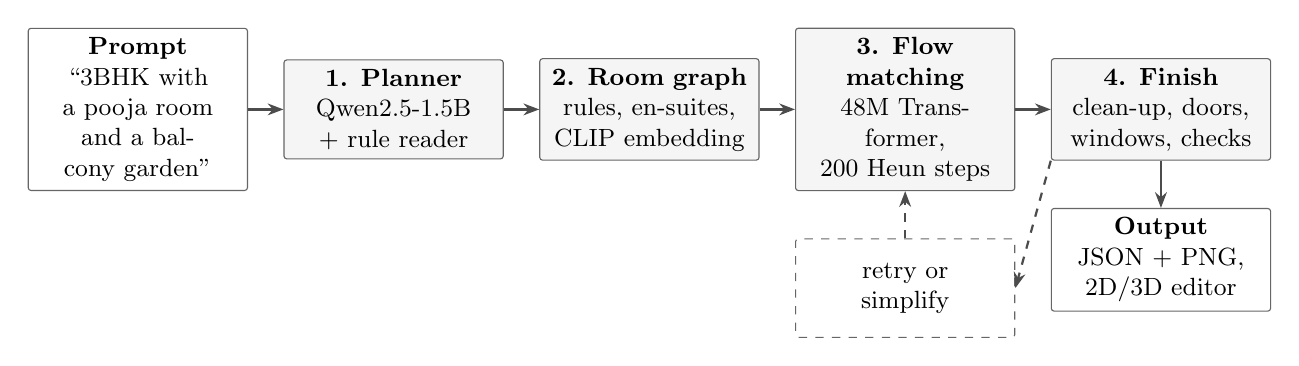
\begin{tikzpicture}[
  node distance=0.45cm,
  box/.style={draw=black!60, fill=black!4, rounded corners=1pt, align=center,
              minimum height=1.25cm, text width=2.55cm, font=\small},
  io/.style={box, fill=white},
  arr/.style={-{Stealth[length=2mm]}, thick, black!70}]
\node[io]  (p)  {\textbf{Prompt}\\ ``3BHK with a pooja room\\and a balcony garden''};
\node[box, right=of p] (pl) {\textbf{1. Planner}\\ Qwen2.5-1.5B\\+ rule reader};
\node[box, right=of pl] (g) {\textbf{2. Room graph}\\ rules, en-suites,\\ CLIP embedding};
\node[box, right=of g] (fm) {\textbf{3. Flow matching}\\ 48M Transformer,\\ 200 Heun steps};
\node[box, right=of fm] (pp) {\textbf{4. Finish}\\ clean-up, doors,\\ windows, checks};
\node[io, below=0.6cm of pp] (out) {\textbf{Output}\\ JSON + PNG,\\ 2D/3D editor};
\node[box, below=0.6cm of fm, fill=white, dashed] (retry) {retry or\\ simplify};
\draw[arr] (p) -- (pl);
\draw[arr] (pl) -- (g);
\draw[arr] (g) -- (fm);
\draw[arr] (fm) -- (pp);
\draw[arr] (pp) -- (out);
\draw[arr, dashed] (pp.south west) -- (retry.east);
\draw[arr, dashed] (retry.north) -- (fm.south);
\end{tikzpicture}
\caption{The FloorPlan AI pipeline. If a plan fails the checks, the system samples
again and, for busy programs, simplifies the request in stages.}
\label{fig:pipeline}
\end{figure}

\subsection{Prompt planner}\label{sec:planner}
The generator knows six room shapes, which we call \emph{slots}: living, kitchen,
bedroom, bathroom, balcony and storage. The planner's job is to turn any sentence
into a list of rooms, each with a display name and a slot.

\paragraph{LLM reader.} Qwen2.5-1.5B-Instruct receives a system prompt that
defines the six slots, two worked examples, and the user's sentence. It replies
with JSON:
\begin{lstlisting}
{"size": "medium", "rooms": [
  {"name": "Living room", "shape": "living",  "count": 1},
  {"name": "Bedroom",     "shape": "bedroom", "count": 3},
  {"name": "Pooja room",  "shape": "storage", "count": 1, "next_to": ["Living room"]},
  {"name": "Balcony garden", "shape": "balcony", "count": 1}]}
\end{lstlisting}
The LLM decides how unusual rooms are drawn (a study or dining room as a
bedroom-sized room, a garden or terrace as a balcony, a pantry or pooja room as
storage). It also chooses a size when none is given, and handles descriptions of
needs such as ``a home for a retired couple who love gardening''. Decoding is
greedy, so the same prompt always gives the same plan.

\paragraph{Rule reader.} A regular-expression reader with a 25-entry room
vocabulary extracts every number the user typed. It understands digits and
number words (``two bedrooms''), ``3BHK'', negation (``no balcony''), plural
mentions without a number, and phrases such as ``every bedroom has an attached
bathroom''.

\paragraph{Merging.} The two readers are combined by three rules:
\begin{enumerate}
  \item A count the user typed always wins over the LLM's count.
  \item When the user lists rooms, the LLM may add only room types the rule reader
        does not know (for example sauna, music room, servant room). It may not add
        extra copies of standard rooms.
  \item If no living room is requested, a central hall is added, because the
        generator places the front door in the living slot.
\end{enumerate}
Counts are then capped at what the model was trained on (for example eight
bedroom-shaped rooms and twenty rooms in total).

\subsection{Room-graph construction}
The generator is conditioned on a room graph: which rooms exist and which open
onto which. We reuse the probabilistic rules of Text2Floorplan for the standard
slots: the kitchen opens onto the living room, bedrooms open onto the living room,
and the second bathroom becomes an en-suite. We then adjust the graph for custom
rooms:
\begin{itemize}
  \item non-sleeping rooms in bedroom slots (dining room, study, gym) get nodes
        that open onto the living room and never own an en-suite;
  \item each room joins the rooms named in its \texttt{next\_to} list, so a dining
        room also opens onto the kitchen and a pantry onto the kitchen;
  \item requested en-suites open only into a sleeping room, the master bedroom
        first, and the remaining bathrooms become shared ones off the living room.
\end{itemize}
The sentence given to CLIP is rebuilt from the slot counts in the format the
model was trained on, for example ``A large 4-bedroom apartment with 3 bathrooms
and 1 balcony.''

\subsection{Conditional flow-matching generator}
Each room is a polygon whose corner count is sampled from dataset statistics, so
a plan is a set of 2D corner points grouped by room. The network is a Transformer
with a hidden width of 512 and 8 attention heads (48.2 million parameters):
\begin{itemize}
  \item two \emph{room-node} layers attend over the room graph using connection
        masks;
  \item four \emph{corner} layers attend over corners within a room, across
        connected rooms, and globally;
  \item the noise level $\sigma$ and the projected CLIP embedding are added
        together and injected through adaptive layer normalisation.
\end{itemize}
The network outputs a velocity for every corner. A second head predicts the
binary digits of each corner coordinate, an idea borrowed from analog
bits~\cite{analogbits} and HouseDiffusion~\cite{housediffusion}. The training
loss is $\mathcal{L}=\mathcal{L}_{\text{flow}}+\lambda\,\mathcal{L}_{\text{bit}}$,
where the bit loss applies only at low noise levels ($\sigma<0.12$) to sharpen the
final coordinates. At inference, 200 Heun steps take the corners from Gaussian
noise to a layout. The model was trained on RPLAN~\cite{rplan} and
ResPlan~\cite{resplan}.

\subsection{Geometry finishing}
The raw corners are turned into a usable plan in five steps:
\begin{enumerate}
  \item corners become room polygons, and generic rules fix small overlaps and gaps;
  \item the plan is scaled to metres from per-size area statistics (small,
        medium or large);
  \item thin slivers are removed;
  \item doors are placed on every connection whose rooms share a wall long enough
        for a door, and the front door is placed on the living room;
  \item windows are placed on exterior walls, and railings on balconies.
\end{enumerate}
If a requested connection cannot be built, it is dropped when every room stays
reachable. Otherwise the cut-off room is connected to a neighbour it touches.

\subsection{Validation, retries and fallback}
A plan is accepted only if it passes four checks:
\begin{itemize}
  \item every room has a clean body;
  \item every room is reachable from the entrance through doors;
  \item walls are orthogonal;
  \item kitchens and bathrooms are at least 2\,m\textsuperscript{2}.
\end{itemize}
A failed plan is sampled again with a new seed. Small programs get 10 attempts.
Programs with 10 or more rooms get 30 attempts in three phases:
\begin{enumerate}
  \item the exact request;
  \item dining and family rooms merged into the living room as open plan;
  \item counts capped at three bathrooms, two outdoor spaces and five bedroom-sized
        rooms.
\end{enumerate}
Each change is written as a note above the plan (Figure~\ref{fig:fallback}).

\subsection{Outputs and editor}
The system writes a PNG preview and a JSON document. The JSON holds:
\begin{itemize}
  \item rooms, with their polygons and labels;
  \item walls, openings (doors and windows) and railings;
  \item areas in m\textsuperscript{2};
  \item the planner's decisions.
\end{itemize}
The JSON opens in a browser editor (Figure~\ref{fig:ui}) with linked 2D and 3D
views. In the editor, walls, doors and windows can be dragged, and areas update
live.

\begin{figure}[H]
\centering
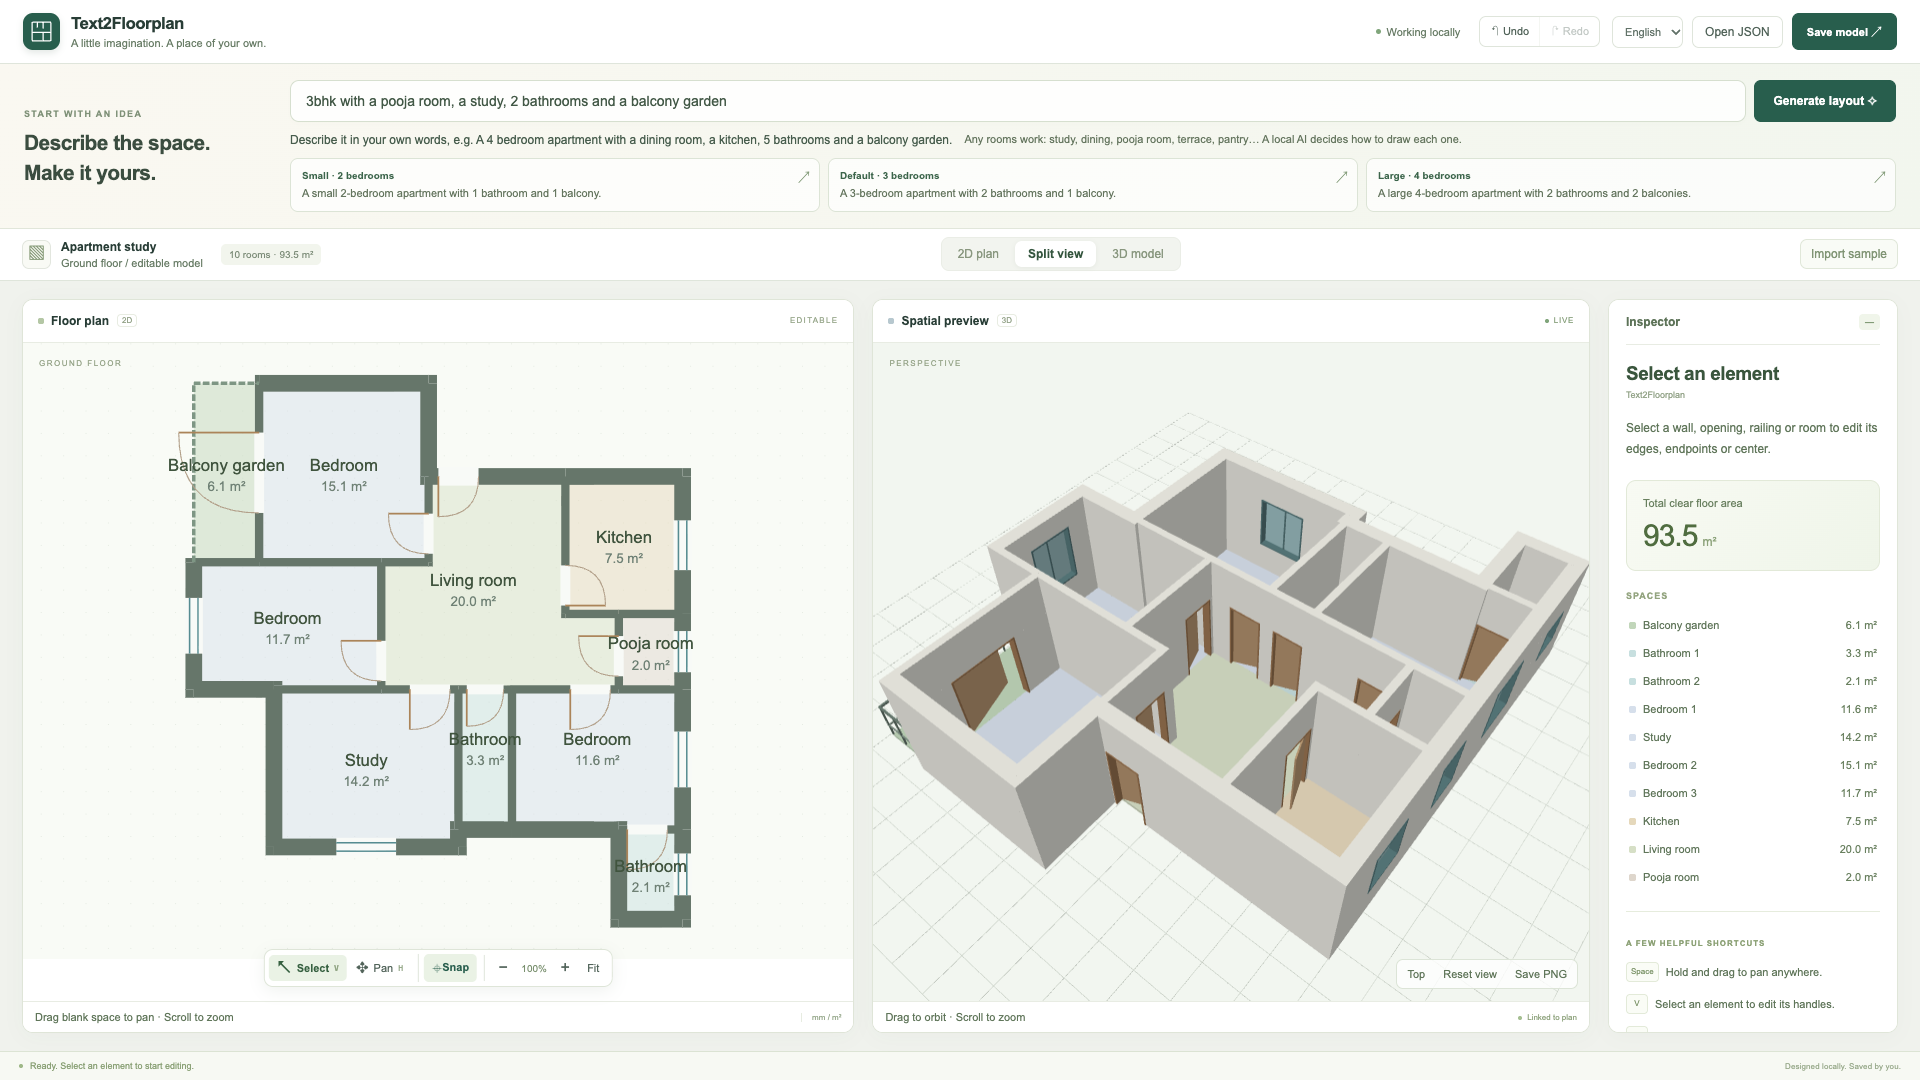
\includegraphics[width=\linewidth]{figures/ui_split.png}
\caption{The browser editor with a generated plan for ``3bhk with a pooja room, a
study, 2 bathrooms and a balcony garden''. Left: editable 2D plan with the user's
room names. Middle: 3D view. Right: room list with areas.}
\label{fig:ui}
\end{figure}

% ================================================================ 5
\section{Implementation}

\subsection{Software and hardware}
\begin{table}[H]
\centering
\caption{Implementation summary.}
\small
\begin{tabularx}{\linewidth}{l X}
\toprule
Language and libraries & Python 3.12, PyTorch 2.11, Hugging Face Transformers 5.14, Shapely, Matplotlib\\
Generator            & Text2Floorplan flow-matching Transformer, 48.2\,M parameters, released checkpoint (193\,MB)\\
Text encoder         & CLIP ViT-L/14 text tower, 768-dimensional pooled output\\
Planner LLM          & Qwen2.5-1.5B-Instruct, float16 on Apple MPS (CPU fallback), greedy decoding\\
Editor               & Local HTTP server with a JavaScript 2D/3D editor\\
Hardware             & Apple M4 laptop, 16\,GB RAM; generation on CPU\\
New code             & \texttt{prompt\_planner.py} (planner, graph rules, fallback, edge repair); changes to the pipeline, backend, CLI and editor; evaluation scripts in \texttt{report/}\\
\bottomrule
\end{tabularx}
\end{table}

\subsection{Datasets}
\begin{itemize}
  \item \textbf{RPLAN}~\cite{rplan}: about 80{,}000 residential plans with room
        types. The released generator was trained on it, and all compared methods
        report results on it. We did not have access to RPLAN.
  \item \textbf{ResPlan}~\cite{resplan}: a vector residential plan dataset, also
        used to train the released generator.
  \item \textbf{Our prompt test set}: 30 hand-written prompts with labelled room
        counts. It covers standard prompts, number words, BHK notation, negation,
        en-suites, and rooms outside the vocabulary (sauna, music room, art studio,
        servant room).
\end{itemize}

\subsection{Code availability and running the system}
The source code, evaluation scripts and this report are available at
\url{https://github.com/lkksharma/FLOORPLAN-generator/tree/main}.
\begin{lstlisting}
# one plan from the command line
.venv/bin/python infer.py --prompt "2 bedroom flat, master bedroom with en-suite, a study and a balcony garden" --device cpu

# browser editor
.venv/bin/python -m web_editor.server --open
\end{lstlisting}

% ================================================================ 6
\section{Experiments and Results}\label{sec:results}

\subsection{Metrics}
\begin{itemize}
  \item \textbf{Count accuracy}: share of the room types mentioned in a prompt
        whose count the planner gets exactly right.
  \item \textbf{GED} (graph edit distance, also called compatibility): the number
        of rooms and connections that differ between the requested room graph and
        the graph of the generated plan~\cite{housediffusion}. For our system it
        counts missing rooms and requested connections whose rooms do not share a
        wall long enough for a door. Doors are placed only on requested
        connections, so extra connections cannot occur.
  \item \textbf{Overlap} and \textbf{\% overlap}~\cite{rlvr}: whether any two
        rooms overlap (by more than 1\% of the smaller room), and the overlapping
        share of the total area. Measured on the raw model output, before
        clean-up.
  \item \textbf{Room ID}~\cite{rlvr}: whether every requested room appears in the
        output.
  \item \textbf{Valid}: whether the finished plan passes all checks without a
        retry.
\end{itemize}

\subsection{Result 1: reading free-form prompts}
Table~\ref{tab:planner} and Figure~\ref{fig:planner} compare four readers on the
30 labelled prompts. The original Text2Floorplan parser only understands digits
directly before ``bedroom'', ``bathroom'' and ``balcony'', so it fails on number
words, BHK notation and every custom room. The LLM alone recognises custom rooms
but miscounts. In one case it gave 3 bedrooms for ``a 4 bedroom apartment''.
Twice it returned malformed JSON, and it sometimes added rooms nobody asked for.
The rule reader counts well but cannot name unknown rooms. Combined, they read
every count correctly and cover every requested room.

\begin{table}[H]
\centering
\caption{Prompt reading on 30 labelled prompts (higher is better).}
\label{tab:planner}
\small
\begin{tabular}{lccc}
\toprule
\textbf{Reader} & \textbf{Count accuracy} & \textbf{Rooms covered} & \textbf{Exact program}\\
\midrule
Original Text2Floorplan parser & 45.7\% & 46.1\% & 13.3\%\\
Qwen2.5-1.5B alone             & 79.8\% & 85.2\% & 56.7\%\\
Our rule reader alone          & 96.1\% & 96.9\% & 83.3\%\\
\textbf{Ours: LLM + rules}     & \textbf{100\%} & \textbf{100\%} & \textbf{100\%}\\
\bottomrule
\end{tabular}
\end{table}

\begin{figure}[H]
\centering
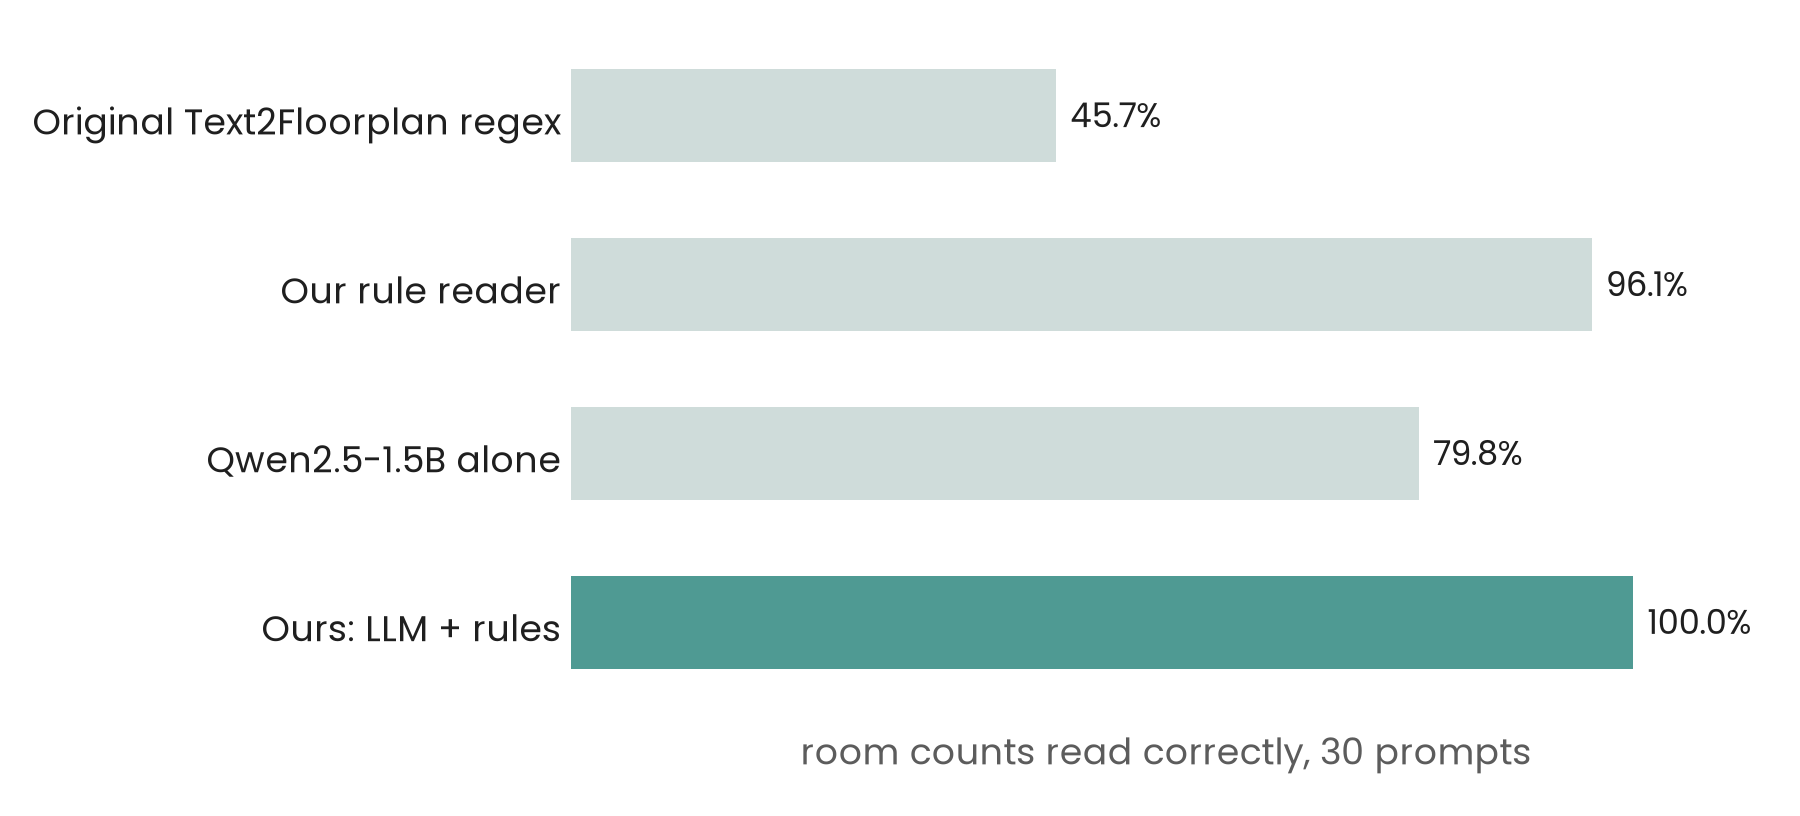
\includegraphics[width=0.78\linewidth]{figures/planner_accuracy.png}
\caption{Share of room counts read correctly by each reader.}
\label{fig:planner}
\end{figure}

The LLM call takes about 14\,s per prompt on the M4, including loading the model.
The test prompts were written by our group, and two bugs in the merge rules were
fixed after looking at failures on this set, so the 100\% figure is optimistic.

\subsection{Result 2: generation quality and speed}
Table~\ref{tab:generation} reports 40 samples: 5 seeds for each of 8 prompts, one
sample per seed, no retries.

\begin{table}[H]
\centering
\caption{Single-sample generation results on CPU.}
\label{tab:generation}
\small
\begin{tabular}{lccc}
\toprule
\textbf{Prompt type} & \textbf{Valid first time} & \textbf{Raw connection recall} & \textbf{Accepted: counts right, GED}\\
\midrule
1 bedroom                         & 100\% (5/5)  & 100\% & 5/5, 0\\
2 bedrooms (2 prompts)            & 60\% (6/10)  & 90\%  & 6/6, 0\\
3 bedrooms (2 prompts)            & 60\% (6/10)  & 95\%  & 6/6, 0\\
4 bedrooms                        & 40\% (2/5)   & 89\%  & 2/2, 0\\
Free-form with extra rooms (2)    & 20\% (2/10)  & 87\%  & 2/2, mean 3\\
\midrule
\textbf{All 40 samples}           & \textbf{52\%} & \textbf{92\%} & \textbf{21/21, mean 0.29}\\
\bottomrule
\end{tabular}
\end{table}

\emph{Raw connection recall} is the share of requested connections that the
generator's geometry already supports before any door repair. Every accepted plan
had exactly the requested rooms. The validity rate falls as plans get busier,
which is why the retry loop exists. The most common rejections are a bathroom
under 2\,m\textsuperscript{2}, a missing doorway, and a thin sliver of a room. One
sample takes about 10\,s on the CPU; with retries a finished plan takes 1.5 to
4 minutes.

\subsection{Comparison with prior work}
To compare on equal terms we reproduced the setting of House-GAN++,
HouseDiffusion and LLM with RLVR: plans with 5, 6, 7 and 8 rooms, one sample per
plan, no retries. We ran 12 samples per size. Figure~\ref{fig:ged} and
Table~\ref{tab:h2h} report every number side by side. Published numbers are
copied from the papers.

\begin{figure}[H]
\centering
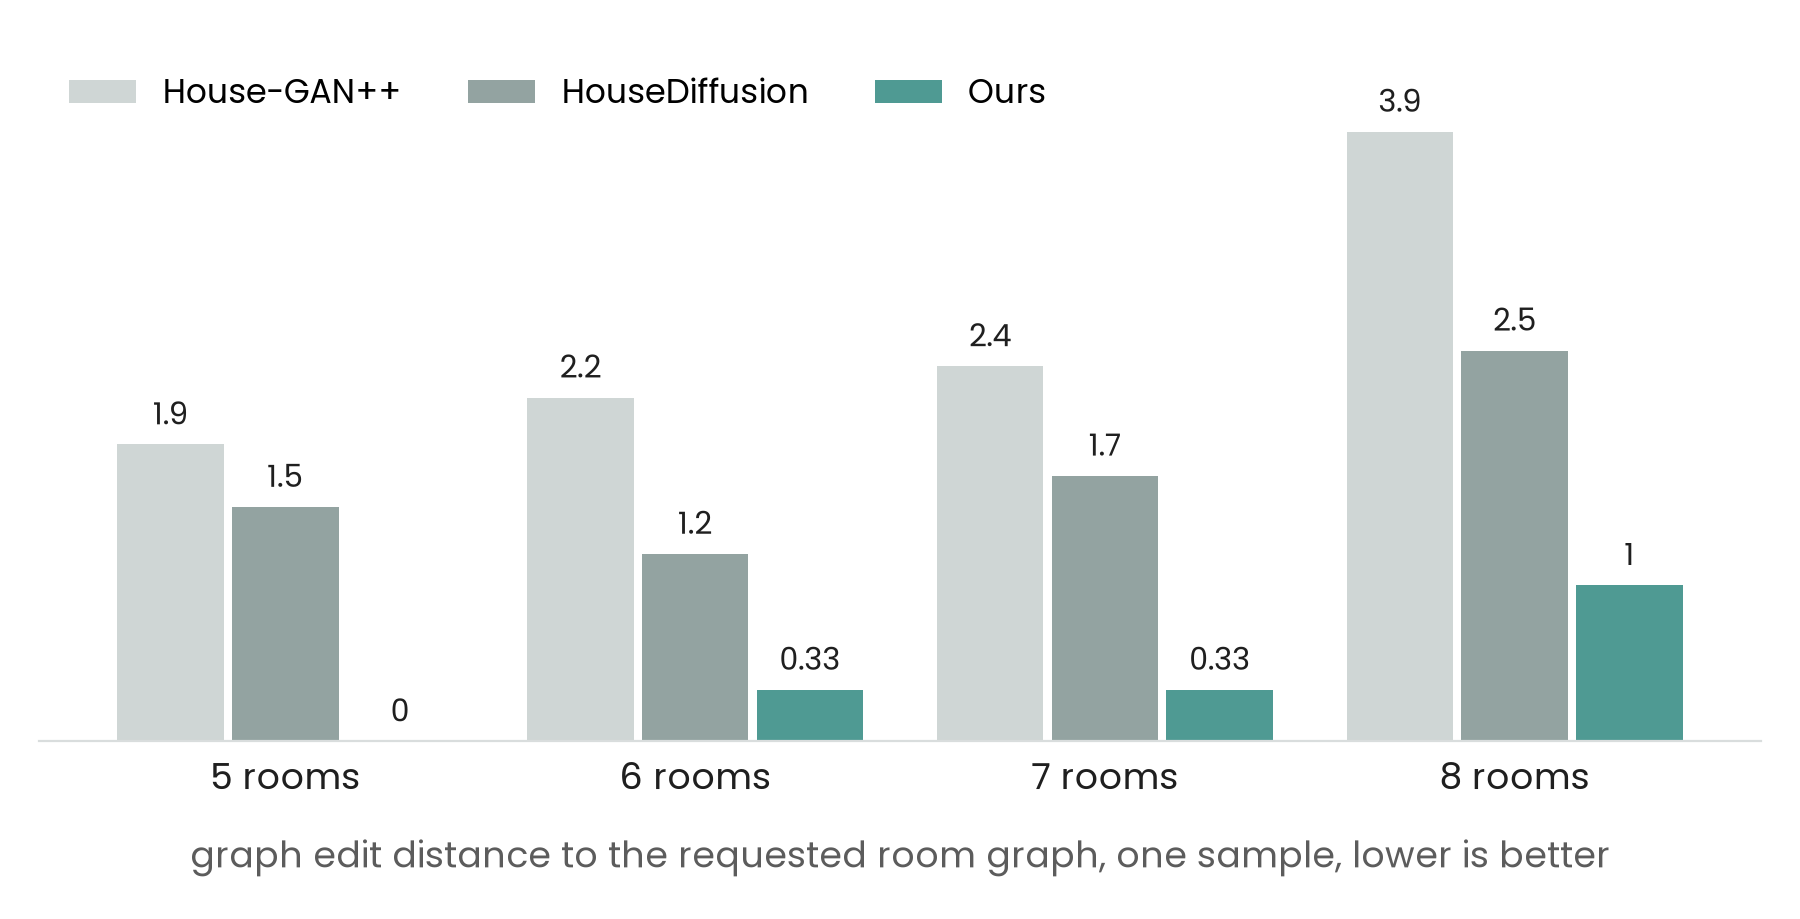
\includegraphics[width=0.82\linewidth]{figures/ged_by_size.png}
\caption{GED between the requested and the generated room graph, by plan size
(lower is better). House-GAN++ and HouseDiffusion values are from
HouseDiffusion~\cite{housediffusion}.}
\label{fig:ged}
\end{figure}

\begin{table}[H]
\centering
\caption{Head-to-head on shared metrics, one sample per plan.}
\label{tab:h2h}
\small
\begin{tabular}{lcccc}
\toprule
\textbf{Metric} & \textbf{House-GAN++}~\cite{housegan2} & \textbf{HouseDiffusion}~\cite{housediffusion} & \textbf{LLM + RLVR}~\cite{rlvr} & \textbf{Ours}\\
\midrule
GED, 5 rooms $\downarrow$ & 1.9 & 1.5 & -- & \textbf{0}\\
GED, 6 rooms $\downarrow$ & 2.2 & 1.2 & -- & \textbf{0.33}\\
GED, 7 rooms $\downarrow$ & 2.4 & 1.7 & -- & \textbf{0.33}\\
GED, 8 rooms $\downarrow$ & 3.9 & 2.5 & 1.89 & \textbf{1.0}\\
Overlap rate, 8 rooms $\downarrow$ & -- & -- & \textbf{0.26} & 1.00\\
\% area overlapping, 8 rooms $\downarrow$ & -- & -- & 0.01 & \textbf{0.005}\\
Room ID, 8 rooms $\uparrow$ & -- & -- & 1.00 & 1.00\\
Parameters & 2\,M & 27\,M & 70\,B & 48\,M + 1.5\,B\\
\bottomrule
\end{tabular}
\end{table}

\paragraph{Reading the comparison.}
\begin{itemize}
  \item \textbf{GED.} Our plans follow the requested room graph more closely than
        every compared method at every size.
  \item \textbf{Overlap.} The raw output overlaps more than the best LLM-based
        method: every 8-room sample had at least one overlap above the 1\%
        threshold. The overlapping area is still small (0.5\% of the plan), and
        the clean-up step removes it, so accepted plans have no overlap.
  \item \textbf{Test data.} Our room graphs come from our own prompts, while the
        papers use RPLAN test graphs. We ran 12 samples per size; they ran
        thousands.
  \item \textbf{FID and IoU.} Realism (FID) and text-to-plan overlap (IoU) both
        need the RPLAN or Tell2Design test sets, which we could not access.
        Table~\ref{tab:published} lists the published values for context only.
\end{itemize}

\begin{table}[H]
\centering
\caption{Other published results, for context (not measured by us).}
\label{tab:published}
\small
\begin{tabular}{lll}
\toprule
\textbf{Method} & \textbf{Metric and setting} & \textbf{Value}\\
\midrule
House-GAN / House-GAN++ / HouseDiffusion & FID, RPLAN 8 rooms $\downarrow$ & 66.4 / 32.9 / 9.5\\
HouseTune / LLM + RLVR & FID, RPLAN 8 rooms $\downarrow$ & 9.0 / 7.0\\
GSDiff & FID, own 757-graph test set $\downarrow$ & 6.82 (HouseDiffusion: 11.87)\\
Graph2Plan / WallPlan / GSDiff & FID, outline-conditioned $\downarrow$ & 8.40 / 9.07 / 7.50\\
Tell2Design / ChatHouseDiffusion & micro IoU, Tell2Design test $\uparrow$ & 54.34 / 60.57\\
Human designers & micro IoU, 100-plan subset $\uparrow$ & 64.67\\
\bottomrule
\end{tabular}
\end{table}

\subsection{Qualitative results}
Figure~\ref{fig:plans} shows two generated plans with custom rooms. In the first,
the study, pooja room and balcony garden are placed and labelled. In the second,
every bedroom has its own en-suite bathroom, and a shared bathroom opens off the
living area. Figure~\ref{fig:fallback} shows the fallback on an over-full request.

\begin{figure}[H]
\centering
\begin{subfigure}{0.48\linewidth}
  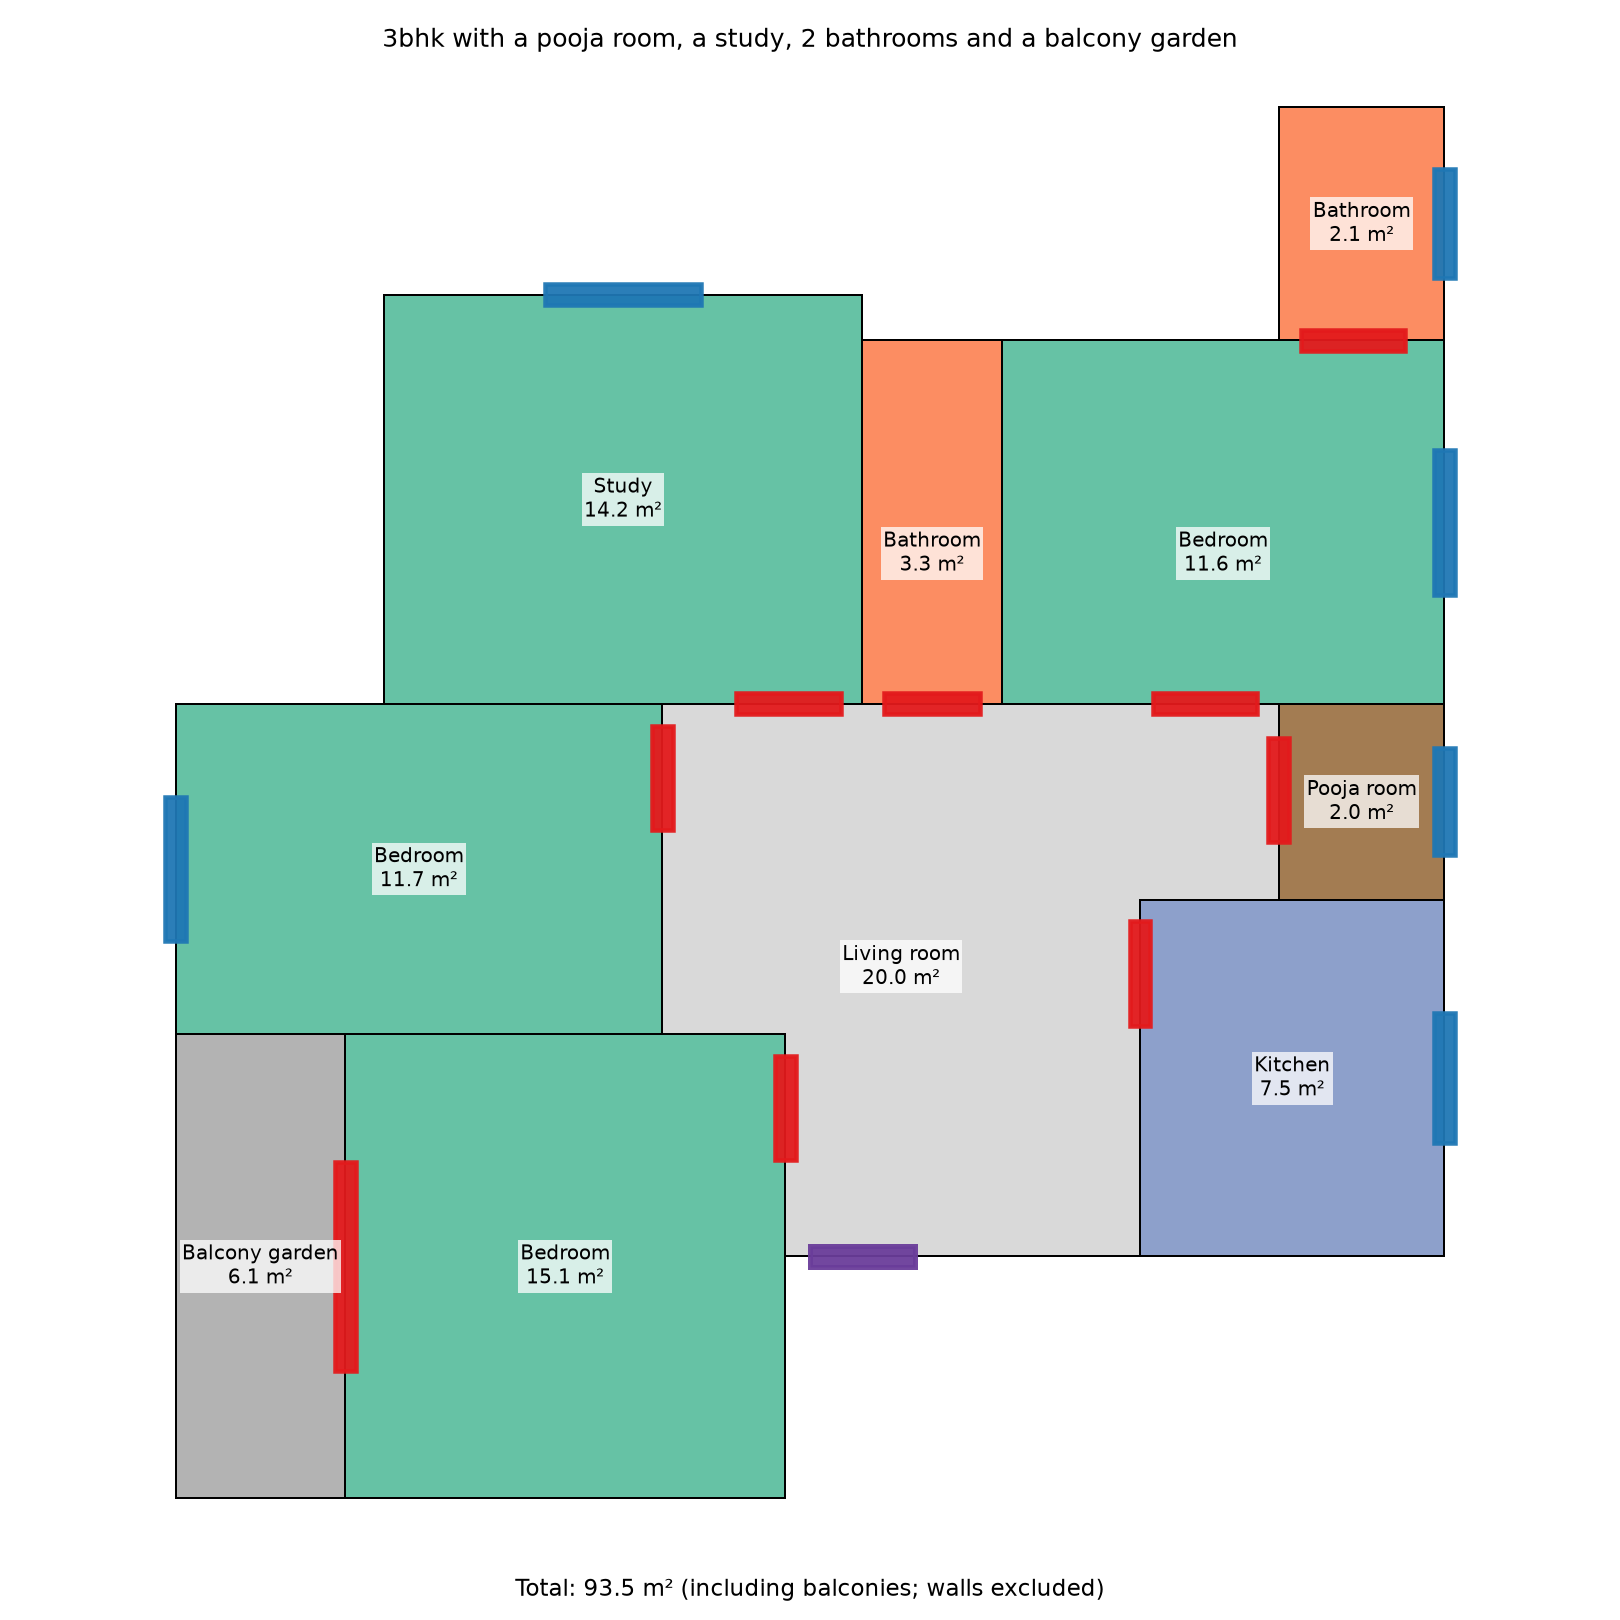
\includegraphics[width=\linewidth]{figures/plan_3bhk_pooja.png}
  \caption{``3bhk with a pooja room, a study, 2 bathrooms and a balcony garden''}
\end{subfigure}\hfill
\begin{subfigure}{0.48\linewidth}
  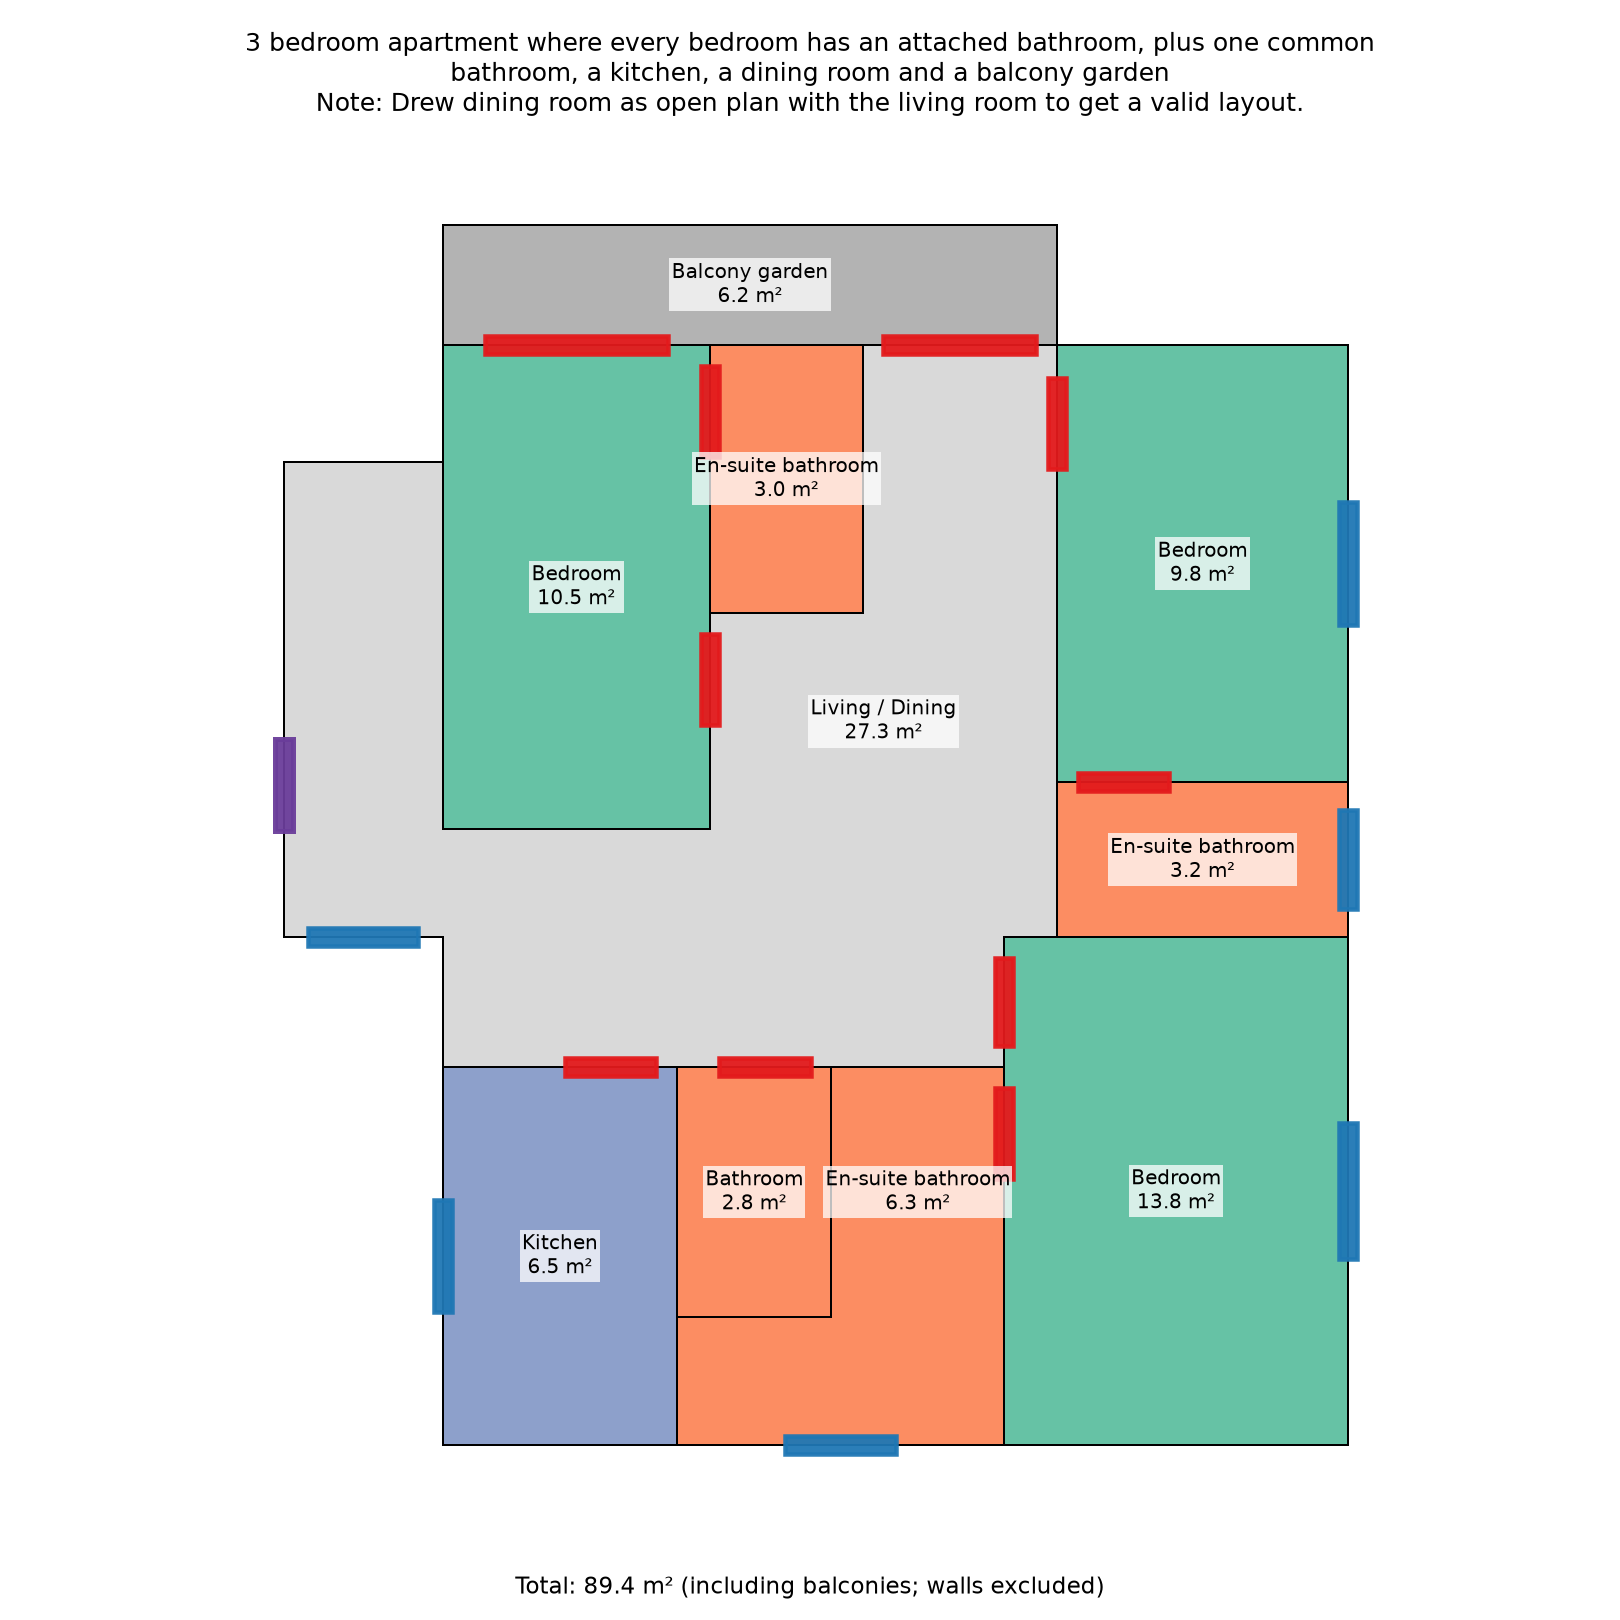
\includegraphics[width=\linewidth]{figures/plan_ensuite.png}
  \caption{``3 bedroom apartment where every bedroom has an attached bathroom,
  plus one common bathroom, a kitchen, a dining room and a balcony garden''}
\end{subfigure}
\caption{Generated plans (PNG previews). Red marks are doors, blue marks are
windows, and the purple mark is the front door.}
\label{fig:plans}
\end{figure}

\begin{figure}[H]
\centering
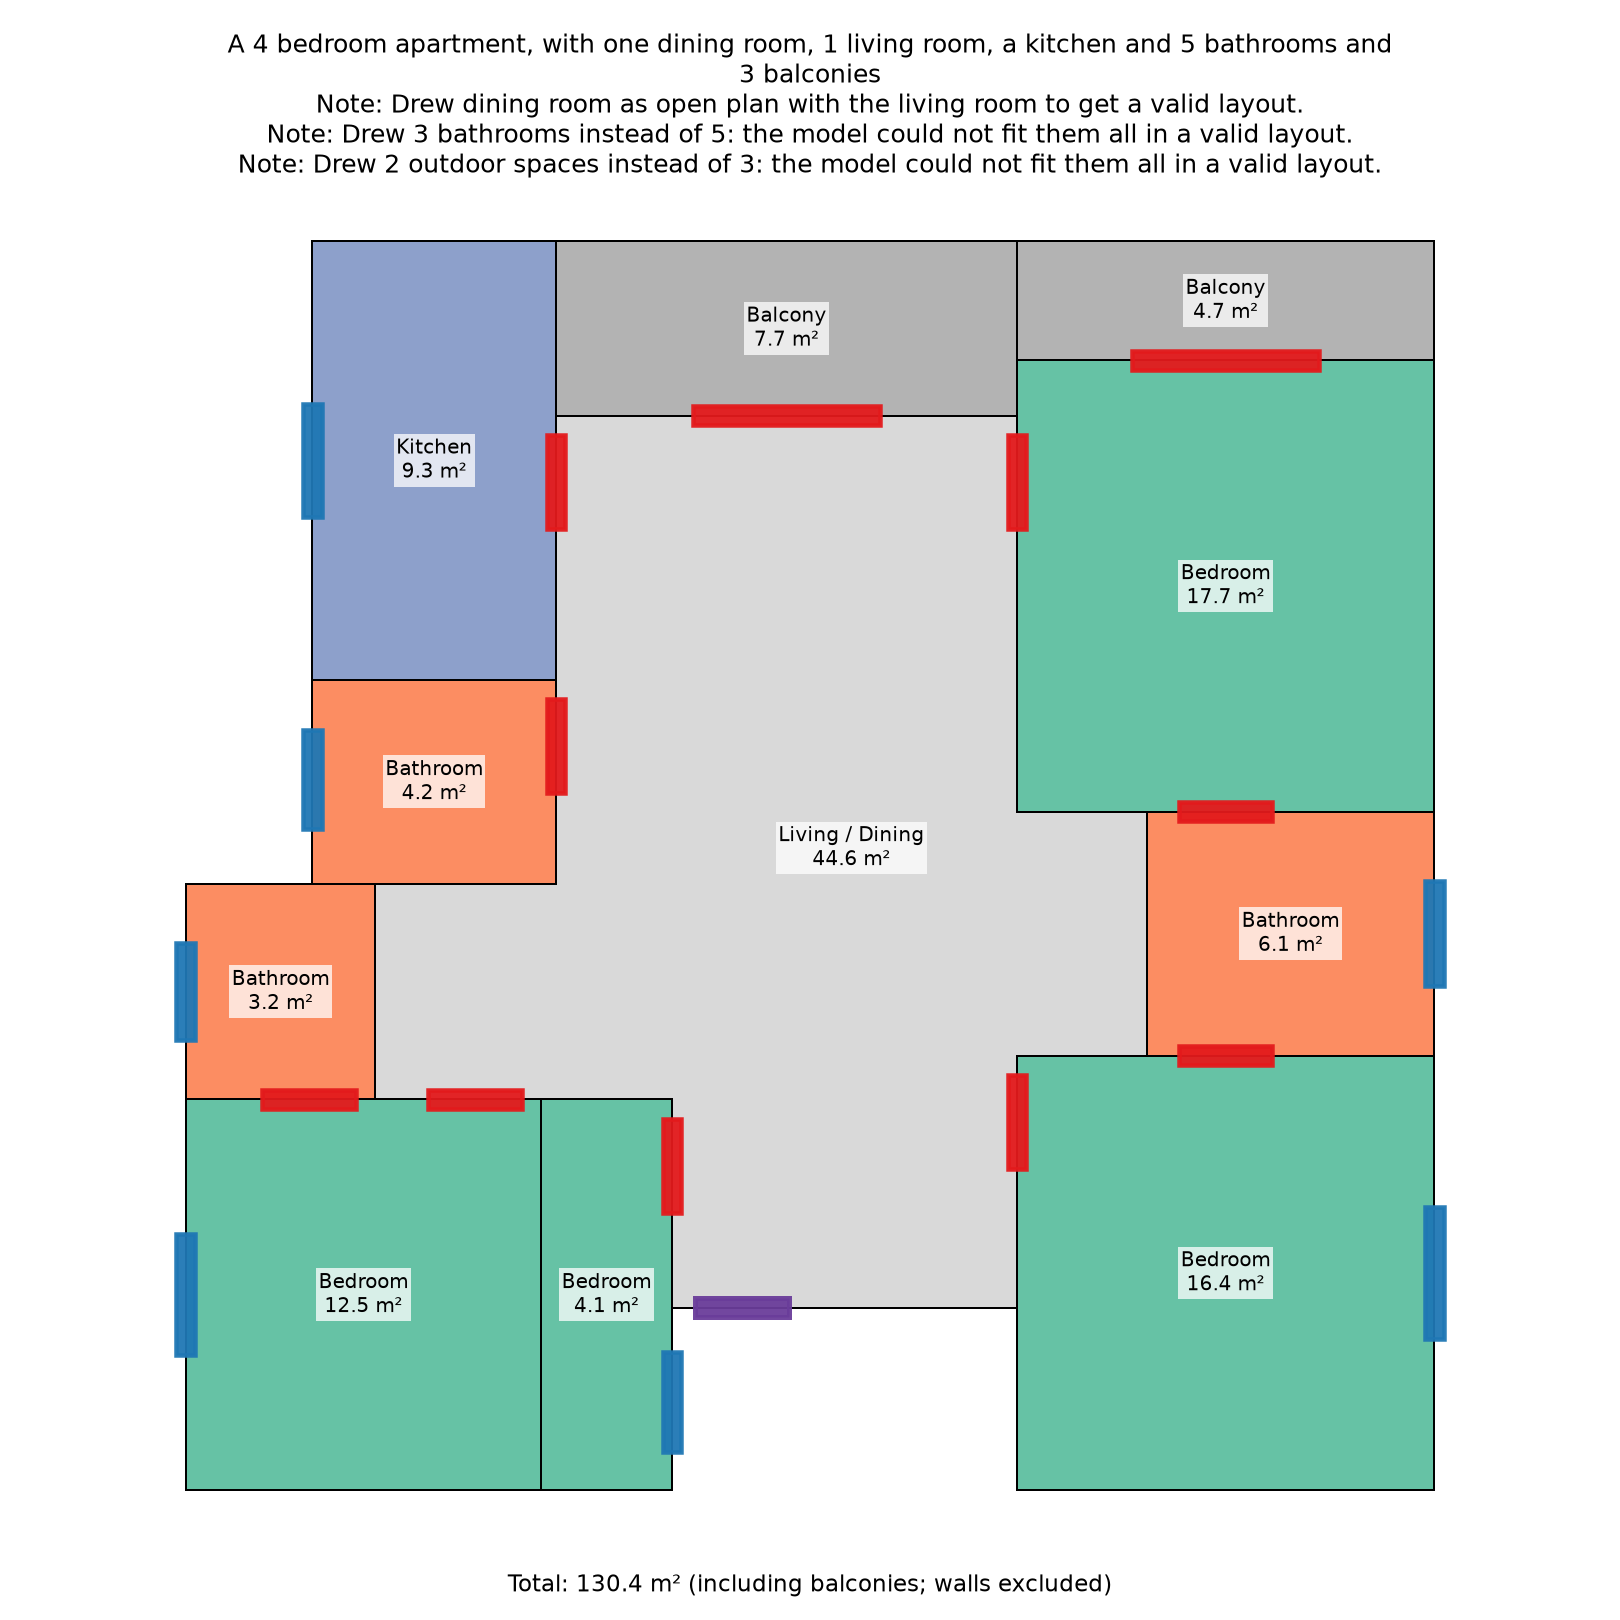
\includegraphics[width=0.55\linewidth]{figures/plan_big_fallback.png}
\caption{``A 4 bedroom apartment, with one dining room, 1 living room, a kitchen
and 5 bathrooms and 3 balconies''. After 20 failed attempts at the exact request,
the system drew the dining area as open plan and capped bathrooms and balconies.
The notes above the plan say so.}
\label{fig:fallback}
\end{figure}

% ================================================================ 7
\section{Discussion and Limitations}
\begin{itemize}
  \item \textbf{The generator was not retrained.} A dining room or study is drawn
        with a bedroom's shape and renamed; the model has no notion of what a
        dining room looks like.
  \item \textbf{Busy programs fail often.} Requests of more than about 12 rooms
        rarely pass the checks. For example, 5 bathrooms and 3 balconies passed
        0 of 32 attempts in our tests. The fallback keeps the system usable but
        changes the request, and it says so on the plan.
  \item \textbf{Raw overlap is high.} Clean-up hides this, but a generator with an
        overlap-aware loss (as in GSDiff's alignment loss or RLVR's rewards) would
        need less repair.
  \item \textbf{Evaluation is small and partly self-made.} The prompt set was
        written by us, and generation was measured on 12--40 samples per setting.
        FID and IoU could not be computed.
  \item \textbf{Speed.} About 10\,s per sample and 14\,s for the LLM on a CPU,
        against under 1\,s per plan for GSDiff on a GPU.
\end{itemize}

% ================================================================ 8
\section{Conclusion and Future Work}
FloorPlan AI shows that a small local language model, used to read the request
rather than to draw the plan, can turn a pretrained floor-plan generator into a
system that accepts plain language. Paired with a rule-based reader and
room-graph rules, it handles custom rooms, attached bathrooms and natural
phrasing, and outputs editable plans with doors, windows and areas on a laptop.
In the setting used by prior work its plans follow the requested room graph more
closely than House-GAN++, HouseDiffusion and an LLM trained with RLVR. Its main
weaknesses are raw room overlap and busy programs.

Future work:
\begin{enumerate}
  \item retrain the generator with more room types, so that dining rooms and
        studies get their own shapes;
  \item add a plot-outline input, as in Graph2Plan and GSDiff;
  \item add an overlap penalty during training;
  \item compute FID and IoU once RPLAN and Tell2Design access is available;
  \item run a user study with architects.
\end{enumerate}

% ================================================================ references
\begin{thebibliography}{99}
\addcontentsline{toc}{section}{References}
\small
\bibitem{housegan} N.~Nauata, K.-H.~Chang, C.-Y.~Cheng, G.~Mori and Y.~Furukawa,
  ``House-GAN: Relational generative adversarial networks for graph-constrained house layout generation,'' in \emph{Proc. ECCV}, 2020.
\bibitem{housegan2} N.~Nauata, S.~Hosseini, K.-H.~Chang, H.~Chu, C.-Y.~Cheng and Y.~Furukawa,
  ``House-GAN++: Generative adversarial layout refinement network towards intelligent computational agent for professional architects,'' in \emph{Proc. CVPR}, 2021.
\bibitem{housediffusion} M.~A.~Shabani, S.~Hosseini and Y.~Furukawa,
  ``HouseDiffusion: Vector floorplan generation via a diffusion model with discrete and continuous denoising,'' in \emph{Proc. CVPR}, 2023.
\bibitem{gsdiff} S.~Hu, W.~Wu, Y.~Wang, B.~Xu and L.~Zheng,
  ``GSDiff: Synthesizing vector floorplans via geometry-enhanced structural graph generation,'' in \emph{Proc. AAAI}, 2025.
\bibitem{graph2plan} R.~Hu, Z.~Huang, Y.~Tang, O.~van~Kaick, H.~Zhang and H.~Huang,
  ``Graph2Plan: Learning floorplan generation from layout graphs,'' \emph{ACM Trans. Graph.}, vol.~39, no.~4, 2020.
\bibitem{wallplan} J.~Sun, W.~Wu, L.~Liu, W.~Min, G.~Zhang and L.~Zheng,
  ``WallPlan: Synthesizing floorplans by learning to generate wall graphs,'' \emph{ACM Trans. Graph.}, vol.~41, no.~4, 2022.
\bibitem{tell2design} S.~Leng, Y.~Zhou, M.~H.~Dupty, W.~S.~Lee, S.~C.~Joyce and W.~Lu,
  ``Tell2Design: A dataset for language-guided floor plan generation,'' in \emph{Proc. ACL}, 2023.
\bibitem{chathousediffusion} Qin \emph{et al.},
  ``ChatHouseDiffusion: Prompt-guided generation and editing of floor plans,'' arXiv:2410.11908, 2024.
\bibitem{housetune} Zong \emph{et al.},
  ``HouseTune: Two-stage floorplan generation with LLM assistance,'' arXiv:2411.12279, 2024.
\bibitem{rlvr} Lara \emph{et al.},
  ``Generative floor plan design with LLMs via reinforcement learning with verifiable rewards,'' NeurIPS 2025 Workshop on UrbanAI; arXiv:2605.14117.
\bibitem{rplan} W.~Wu, X.-M.~Fu, R.~Tang, Y.~Wang, Y.-H.~Qi and L.~Liu,
  ``Data-driven interior plan generation for residential buildings,'' \emph{ACM Trans. Graph.}, vol.~38, no.~6, 2019.
\bibitem{resplan} ResPlan residential floor-plan dataset, \url{https://github.com/m-agour/ResPlan}.
\bibitem{t2f} Text2Floorplan: text to editable floor plans with flow matching, \url{https://github.com/simerionon/Text2Floorplan}, commit 12d00c1.
\bibitem{flowmatching} Y.~Lipman, R.~T.~Q.~Chen, H.~Ben-Hamu, M.~Nickel and M.~Le,
  ``Flow matching for generative modeling,'' in \emph{Proc. ICLR}, 2023.
\bibitem{rectifiedflow} X.~Liu, C.~Gong and Q.~Liu,
  ``Flow straight and fast: Learning to generate and transfer data with rectified flow,'' in \emph{Proc. ICLR}, 2023.
\bibitem{edm} T.~Karras, M.~Aittala, T.~Aila and S.~Laine,
  ``Elucidating the design space of diffusion-based generative models,'' in \emph{Proc. NeurIPS}, 2022.
\bibitem{ddpm} J.~Ho, A.~Jain and P.~Abbeel,
  ``Denoising diffusion probabilistic models,'' in \emph{Proc. NeurIPS}, 2020.
\bibitem{analogbits} T.~Chen, R.~Zhang and G.~Hinton,
  ``Analog bits: Generating discrete data using diffusion models with self-conditioning,'' in \emph{Proc. ICLR}, 2023.
\bibitem{clip} A.~Radford \emph{et al.},
  ``Learning transferable visual models from natural language supervision,'' in \emph{Proc. ICML}, 2021.
\bibitem{qwen25} Qwen Team, ``Qwen2.5 technical report,'' arXiv:2412.15115, 2024.
\end{thebibliography}

\end{document}
